% Copyright 2004 by Till Tantau <tantau@users.sourceforge.net>.
%
% In principle, this file can be redistributed and/or modified under
% the terms of the GNU Public License, version 2.
%
% However, this file is supposed to be a template to be modified
% for your own needs. For this reason, if you use this file as a
% template and not specifically distribute it as part of a another
% package/program, I grant the extra permission to freely copy and
% modify this file as you see fit and even to delete this copyright
% notice. 

\documentclass{beamer}
\usepackage{subfig}

% There are many different themes available for Beamer. A comprehensive
% list with examples is given here:
% http://deic.uab.es/~iblanes/beamer_gallery/index_by_theme.html
% You can uncomment the themes below if you would like to use a different
% one:
%\usetheme{AnnArbor}
%\usetheme{Antibes}
%\usetheme{Bergen}
%\usetheme{Berkeley}
%\usetheme{Berlin}
%\usetheme{Boadilla}
%\usetheme{boxes}
%\usetheme{CambridgeUS}
%\usetheme{Copenhagen}
%\usetheme{Darmstadt}
%\usetheme{default}
%\usetheme{Frankfurt}
%\usetheme{Goettingen}
%\usetheme{Hannover}
%\usetheme{Ilmenau}
%\usetheme{JuanLesPins}
%\usetheme{Luebeck}
\usetheme{Madrid}
%\usetheme{Malmoe}
%\usetheme{Marburg}
%\usetheme{Montpellier}
%\usetheme{PaloAlto}
%\usetheme{Pittsburgh}
%\usetheme{Rochester}
%\usetheme{Singapore}
%\usetheme{Szeged}
%\usetheme{Warsaw}

\title{Capsule Networks}

% A subtitle is optional and this may be deleted
\subtitle{Dynamic Routing Between Capsules}

\author{Louis (Yiqing) Luo}
% - Give the names in the same order as the appear in the paper.
% - Use the \inst{?} command only if the authors have different
%   affiliation.

\institute[University of Toronto] % (optional, but mostly needed)


\date{July 6th, 2018}
% - Either use conference name or its abbreviation.
% - Not really informative to the audience, more for people (including
%   yourself) who are reading the slides online


% Delete this, if you do not want the table of contents to pop up at
% the beginning of each subsection:
\AtBeginSubsection[]
{
  \begin{frame}<beamer>{Outline}
    \tableofcontents[currentsection,currentsubsection]
  \end{frame}
}

% Let's get started
\begin{document}

\begin{frame}
  \titlepage
\end{frame}

\begin{frame}{Outline}
  \tableofcontents
  % You might wish to add the option [pausesections]
\end{frame}

% Section and subsections will appear in the presentation overview
% and table of contents.
\section{Capsule Network Intuition}
\subsection{Capsule Network - Intuition}

\begin{frame}{Capsule Network - Intuition}
  \begin{itemize}
  \item {
    Drawbacks of CNN currently constructed
  }
      \begin{enumerate}
        \item
          Sub-sampling loses the precise spatial relationships between higher-level parts such as a nose and a mouth. The precise spatial relationships are needed for identity recognition 
            \begin{itemize}
                \item
                But overlapping the sub-sampling pools mitigates this. 
            \end{itemize}
        \item{
        They cannot extrapolate their understanding of
geometric relationships to radically new viewpoints.}
        \item Discard (invariant) instead of disentangle (equivariant). Knowledge should be invariant, not activities inside networks.
        \end{enumerate}

  \end{itemize}
  
  \begin{figure}
      \centering
      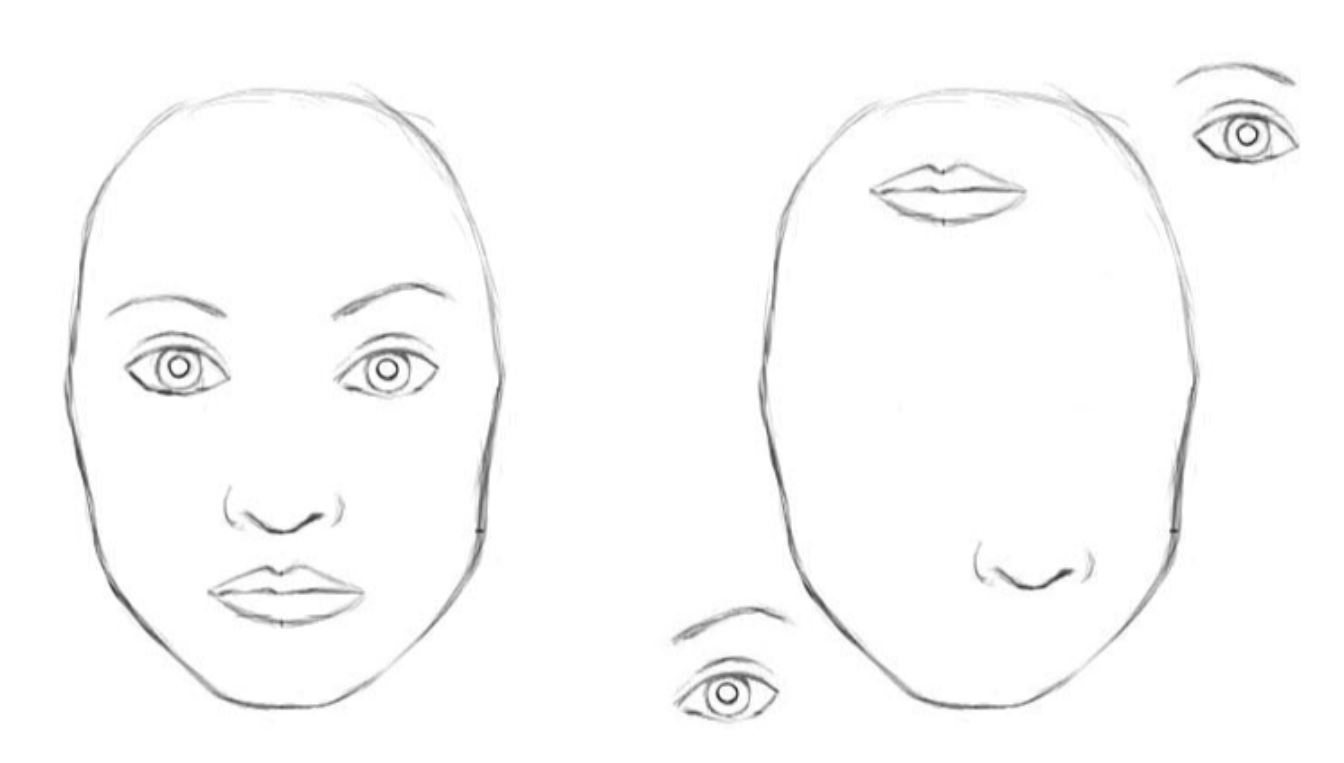
\includegraphics[scale = 0.15]{faces.JPG}
  \end{figure}
  
  \pause % The slide will pause after showing the first item
  \noindent\rule{\textwidth}{1pt}
    \begin{quote}
      Hinton: “The pooling operation used in convolutional neural networks is a big mistake and the fact that it works so well is a disaster.”
  \end{quote}
\end{frame}

\subsection{Better Representation of Images: Inverse Graphics}
% You can reveal the parts of a slide one at a time
% with the \pause command:
\begin{frame}{Better Representation of Images: Inverse Graphics}
  \begin{itemize}
  \item {
    Hinton claims that brain deconstruct hierarchy representation of visual information and tries to match patterns and relationships already learned.
  }
      \begin{itemize}
        \item{representation of objects in brain does not depend on view angles.}
      \end{itemize}
  \item {   
    3D graphics: relationships between 3D objects can be represented by poses
  }
  % You can also specify when the content should appear
  % by using <n->:
  \item {
    Hinton: correct classification and recognition requires preservation of hierarchy pose relationship between objects
  }
  % or you can use the \uncover command to reveal general
  % content (not just \items):
  \end{itemize}
  \begin{figure}[h]
    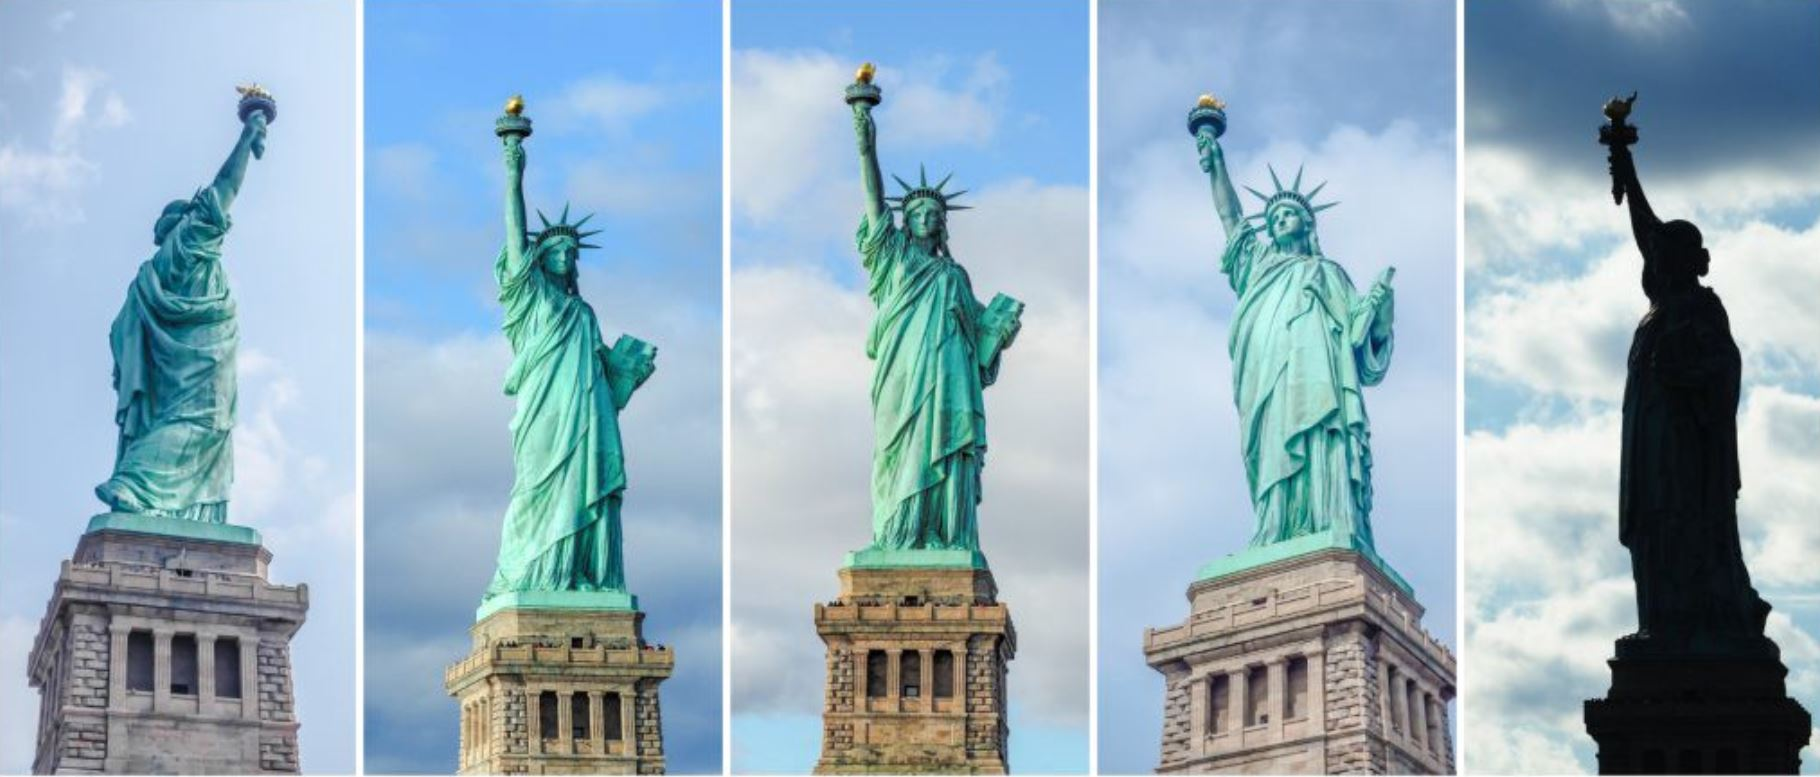
\includegraphics[scale=0.3]{statues.JPG}
    \end{figure}
\end{frame}

\begin{frame}{Better Representation of Images: Inverse Graphics}
    \begin{itemize}
        \item Inverse Graphics is widely employed in computer vision.
        \item Uses hierarchical models in which spatial structure is modeled by matrices that represent the transformation from a coordinate frame embedded in the whole to a coordinate frame embedded in each part
        \item matrices are viewpoint invariant.
    \end{itemize}
    
    
    \begin{figure}[h]
        \centering
        \subfloat[]{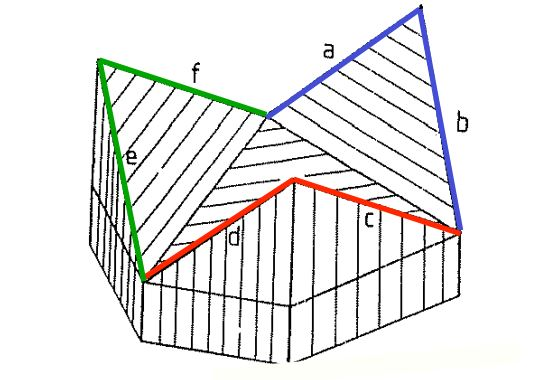
\includegraphics[height=3cm,width=4cm]{crown.JPG}}\qquad
  \subfloat[]{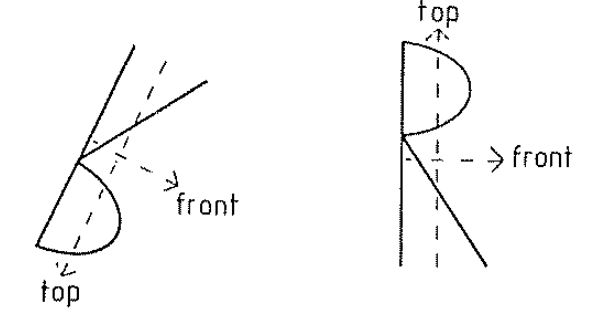
\includegraphics[height=3cm,width=4cm]{r.JPG}}
        \label{}

        
    \end{figure}
\end{frame}

\section{Capsules}
\subsection{What are capsules}

\begin{frame}{What are capsules}
    \begin{itemize}
    \item{
    each capsule will learn to recognize an implicitly defined visual entity over a limited domain of viewing conditions and deformations}
    \item {
    Outputs:
    }
    \begin{enumerate}
        
        \item probability that the entity is within its limited domain (length of the vector does note change)
        \item a set of instantiation parameters (eg. pose, lighting, possible deformations relative to implicitly defined canonical version of entities) (orientation of the vector changes)
        
    \end{enumerate}
    
    \centering
    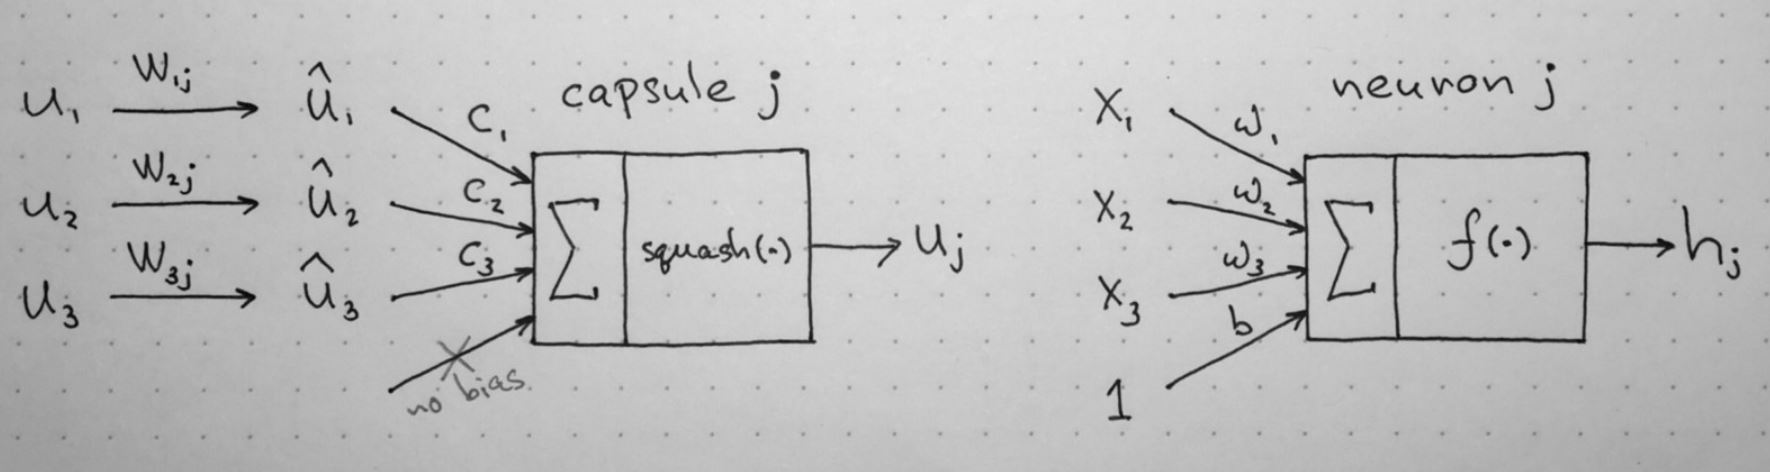
\includegraphics[scale = 0.4]{capsules.JPG}
    
    \end{itemize}
\end{frame}

\begin{frame}{Coincidence Filtering}
    \begin{itemize}
        \item capsules receive multi-dimensional prediction vectors from capsules in layer below and look for tight predictions
        \item Outputs can also be described as:
        \begin{enumerate}
            
            \item probability that the entity exist within its domain
            \item Center of gravity of the cluster = generalized pose
        \end{enumerate}
        \item good at filtering noise because coincidences rarely happens in high dimension space
    \end{itemize}
    \begin{figure}
        \centering
        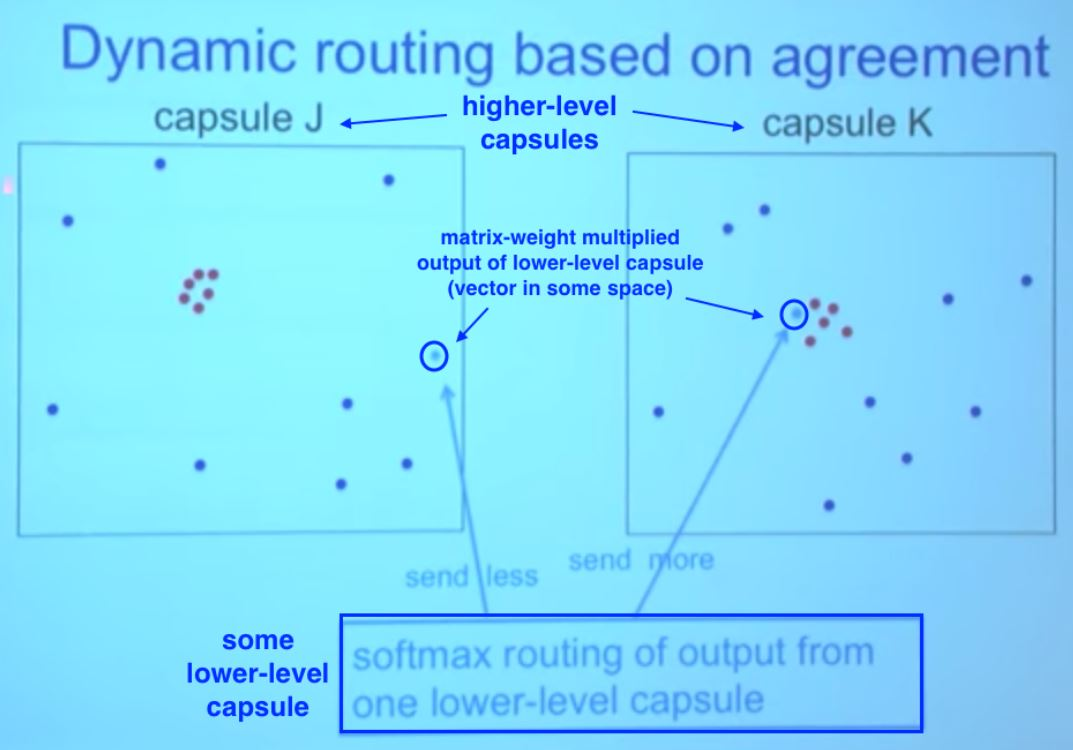
\includegraphics[scale = 0.4]{dr_agreement.JPG}
    \end{figure}
\end{frame}


\subsection{Capsule vs Neurons}
\begin{frame}{Capsule vs Neurons}

    \begin{figure}
        \centering
        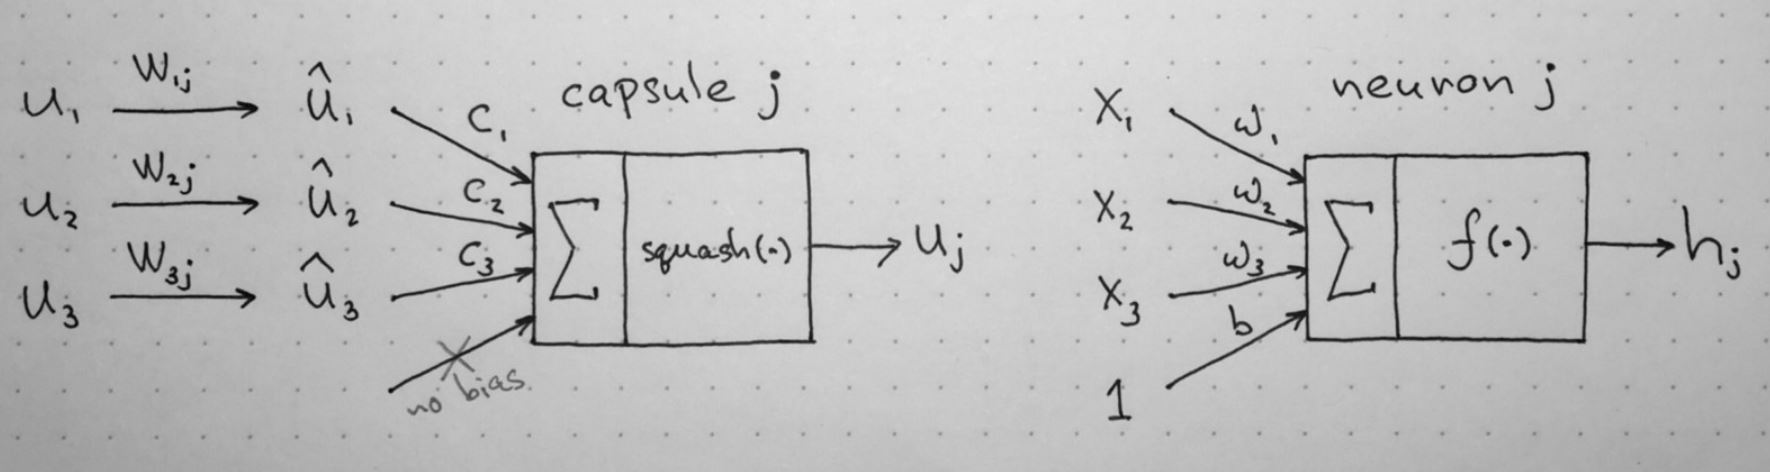
\includegraphics[scale = 0.4]{capsules.JPG}
    
        \centering
        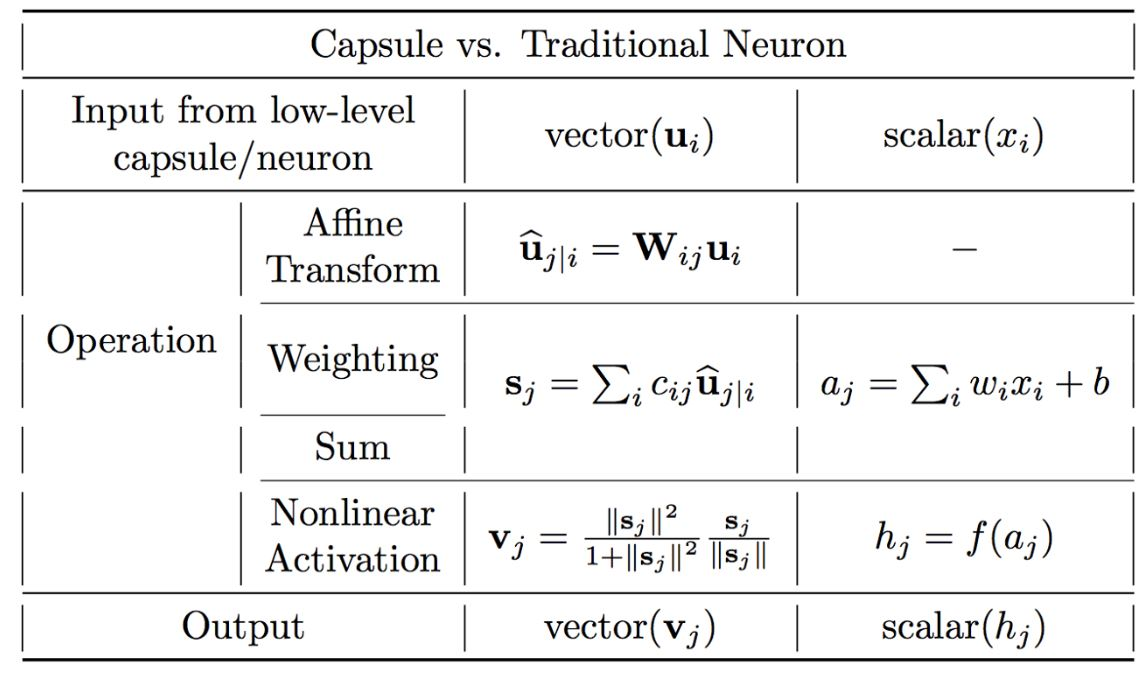
\includegraphics[scale = 0.5]{capsule_calculations.JPG}
    \end{figure}
\end{frame}



%\subsection{Matrix Multiplication on Input Vectors}
\begin{frame}{Matrix Multiplication on Input Vectors}
    \begin{itemize}
        \item inputs $u_1$, $u_2$, $u_3$ contains probability of features and their poses
        \item eg. for detecting a nose from a face:
            \begin{itemize}
                \item $W_{ij}$ encodes relationship from $i_{th}$ feature (nose) to $j_{th}$ feature (face)
            \end{itemize}
            
    \end{itemize}    
    
    \centering
    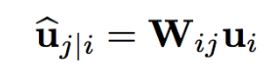
\includegraphics[scale=1]{capsule_1.JPG}
\end{frame}

%\subsection{Scalar Weighting}
\begin{frame}{Scalar Weighting}
    \begin{itemize}
        \item measures the affinity between low level capsules and high level capsules
        \item $c_{ij}$ is adjusted each iteration by dynamic routing
    \end{itemize}
    \begin{figure}
        \centering
        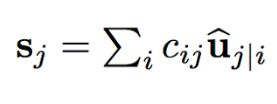
\includegraphics{capsule_2.JPG}
    \end{figure}
\end{frame}

%\subsection{Scalar Weighting - Dynamic Routing}
\begin{frame}{Scalar Weighting - Dynamic Routing}
    \begin{itemize}
        \item decides how to send output vector to higher level capsule j by changing $c_{ij}$ 
        \item important properties of $c_{ij}$
        \begin{enumerate}
            \item $c_{ij}$ non-negative scalar
            \item $\Sigma_j c_{ij} = 1 $ for all i
            \item \# of weights for the vector $c_i$ = \# of higher level capsules
            \item determined by iterative dynamic routing algorithm
        \end{enumerate}
    \end{itemize}
    \begin{figure}
        \centering
        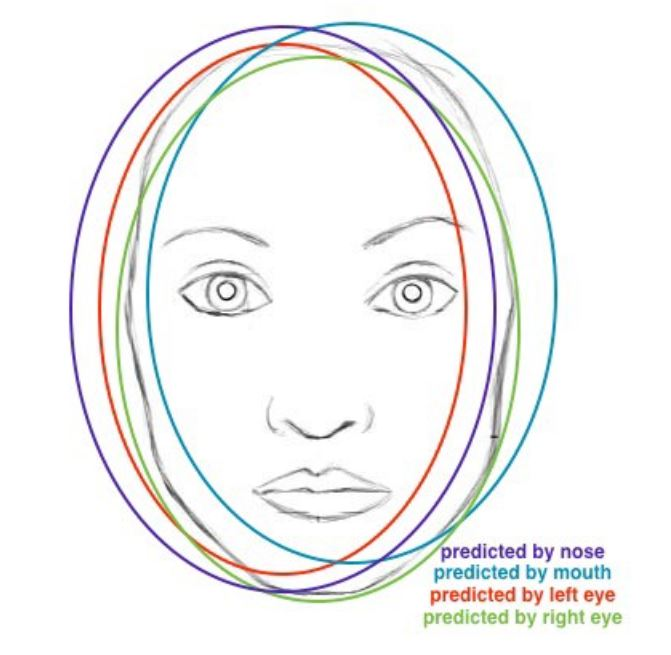
\includegraphics[scale=0.5]{overla.JPG}
    \end{figure}
\end{frame}

%\subsection{Dynamic Routing - Algorithm}
\begin{frame}{Dynamic Routing - Algorithm}
    \begin{figure}[h]
        \centering
        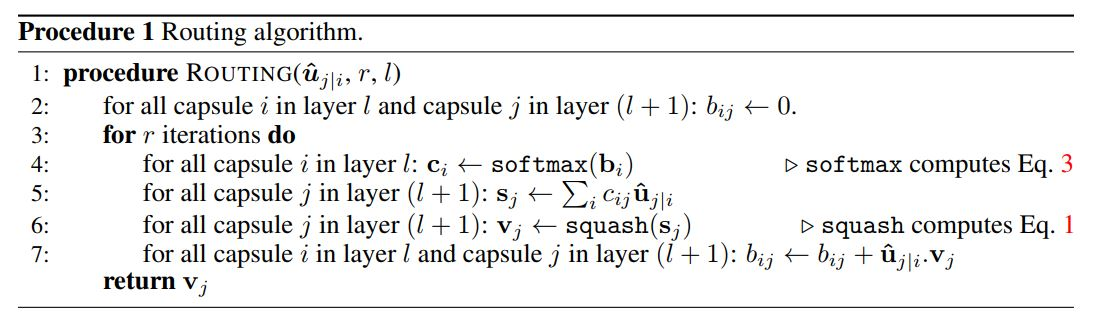
\includegraphics[scale=0.8]{algorithm.JPG}
    \end{figure}
    \begin{figure}[h]
        \centering
        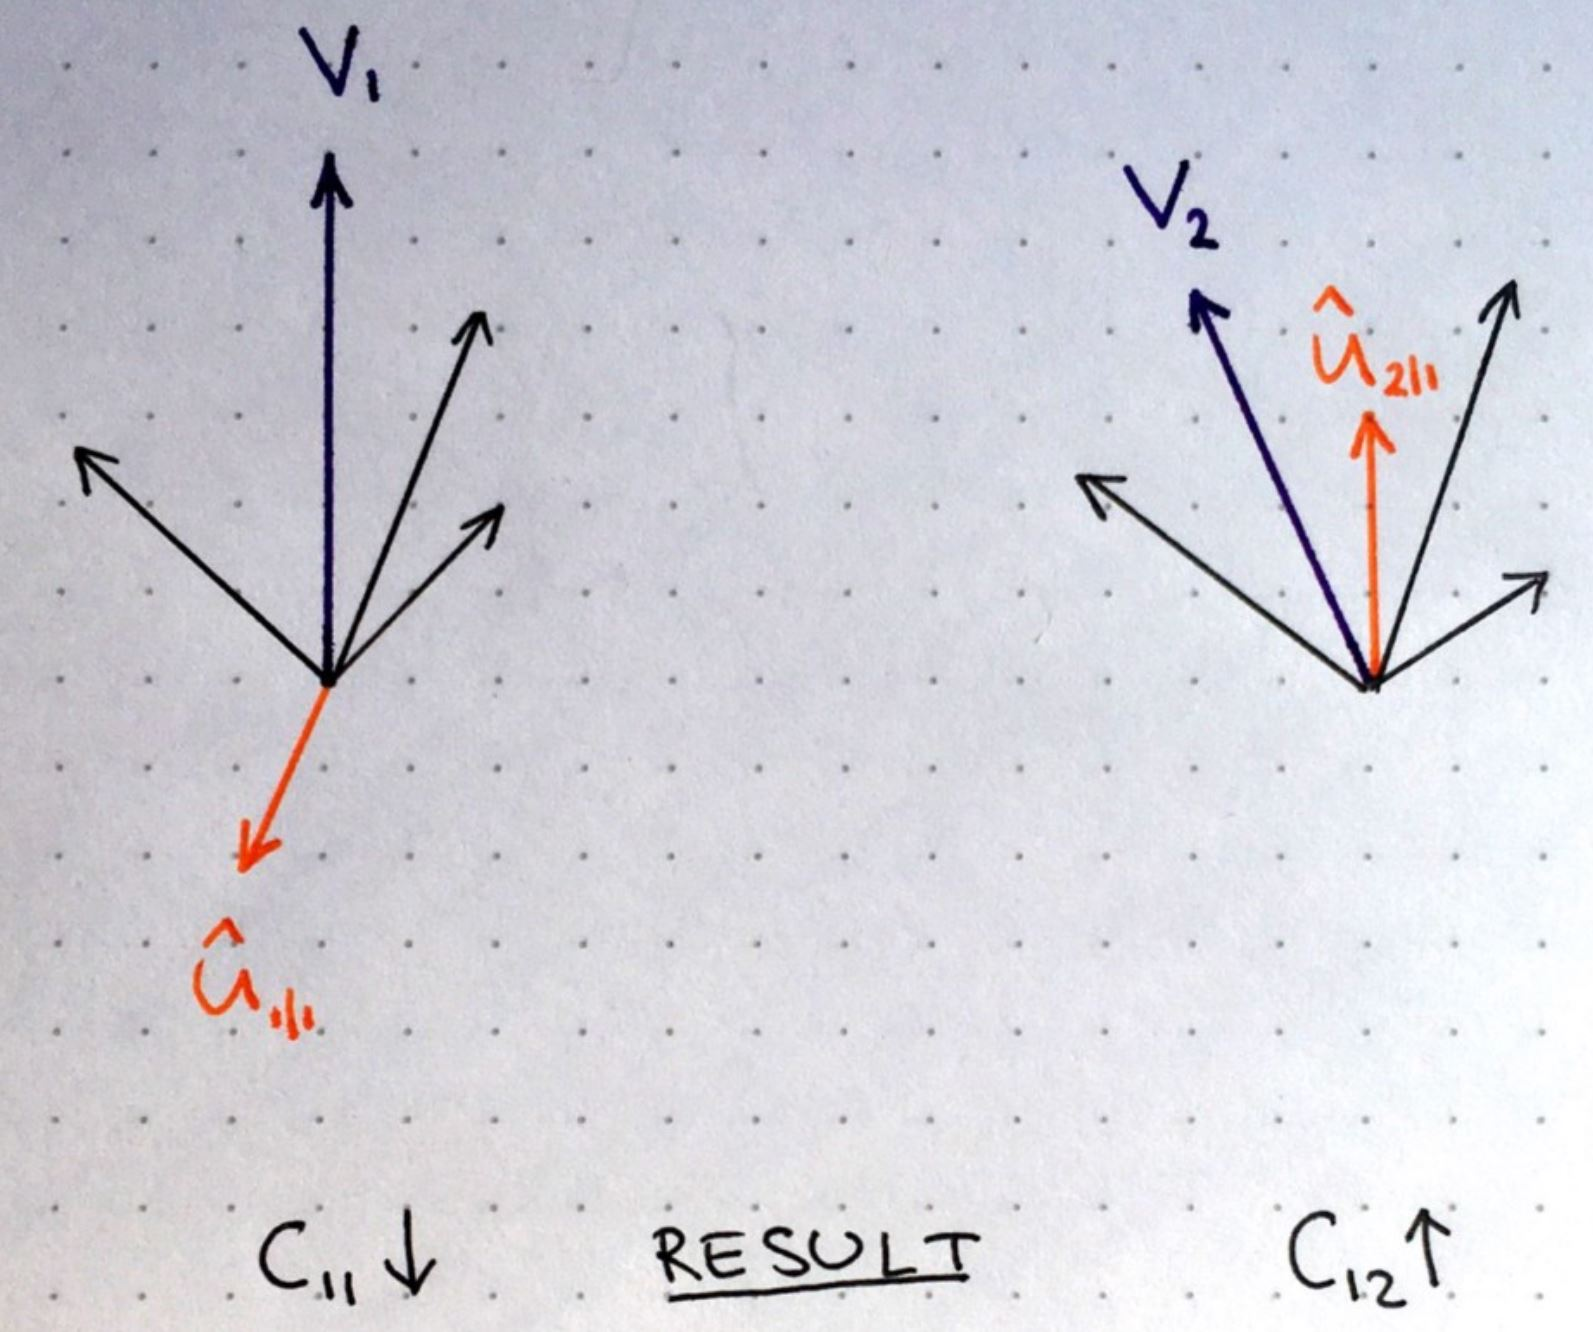
\includegraphics[scale = 0.15]{dr_dot.JPG}
        \end{figure}
\end{frame}

%\subsection{Squash for Non-Linearity}
\begin{frame}{Squash for Non-Linearity}
\begin{figure}
    \centering
    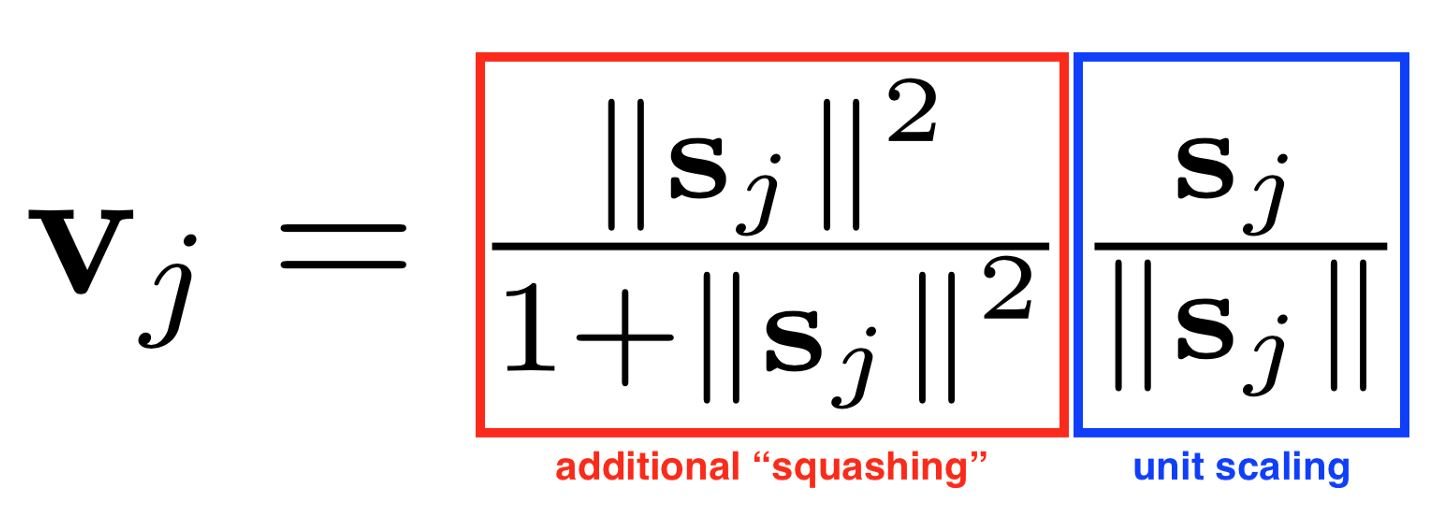
\includegraphics[scale=0.5]{capsule_3.JPG}
\end{figure}
\end{frame}

\subsection{Properties of capsules}
\begin{frame}{Properties of capsules}
    \begin{enumerate}
    \item {
        probability = invariant}
    \begin{itemize}
        \item does note change for possible appearances in manifold within limited domain covered by capsule
    \end{itemize}
    
    \item {
    instantiation parameters = equivariant}
    \begin{itemize}
        \item change in viewing conditions, position etc. change correspondingly over the appearance manifold
        \begin{itemize}
            \item face is centered around the nose
            \item nose is 10 times smaller than the face
            \item same orientation in space
        \end{itemize}
    \end{itemize}
    
    \end{enumerate}
    \centering
    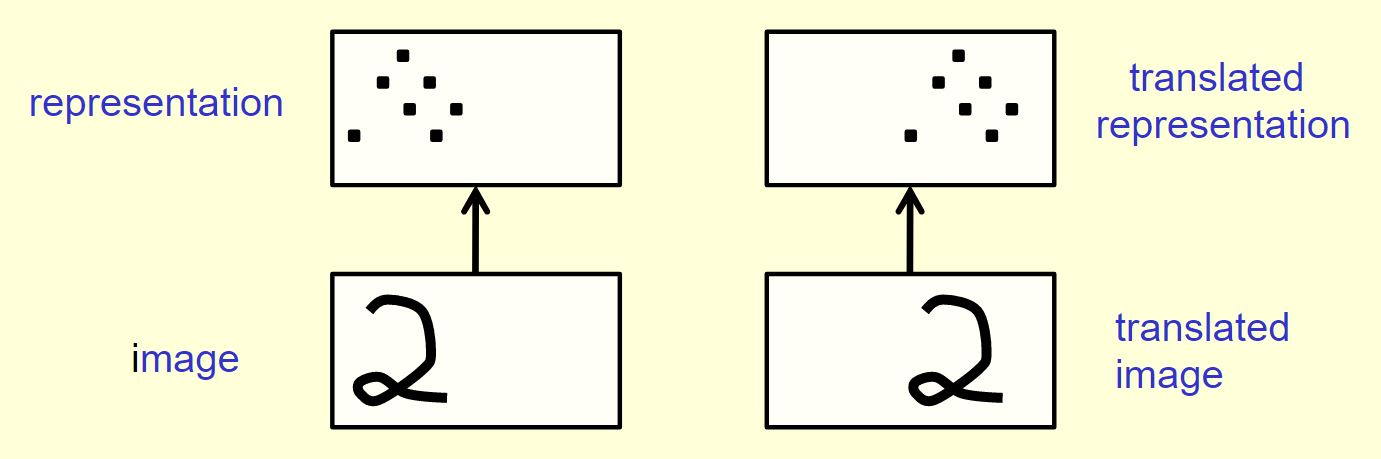
\includegraphics[scale=0.5]{equivariance.JPG}
\end{frame}

\section{Capsule Network}
\subsection{Capsule Network Encoder Architecture}
\begin{frame}{Capsule Network Encoder Architecture}
    \begin{figure}
        \centering
        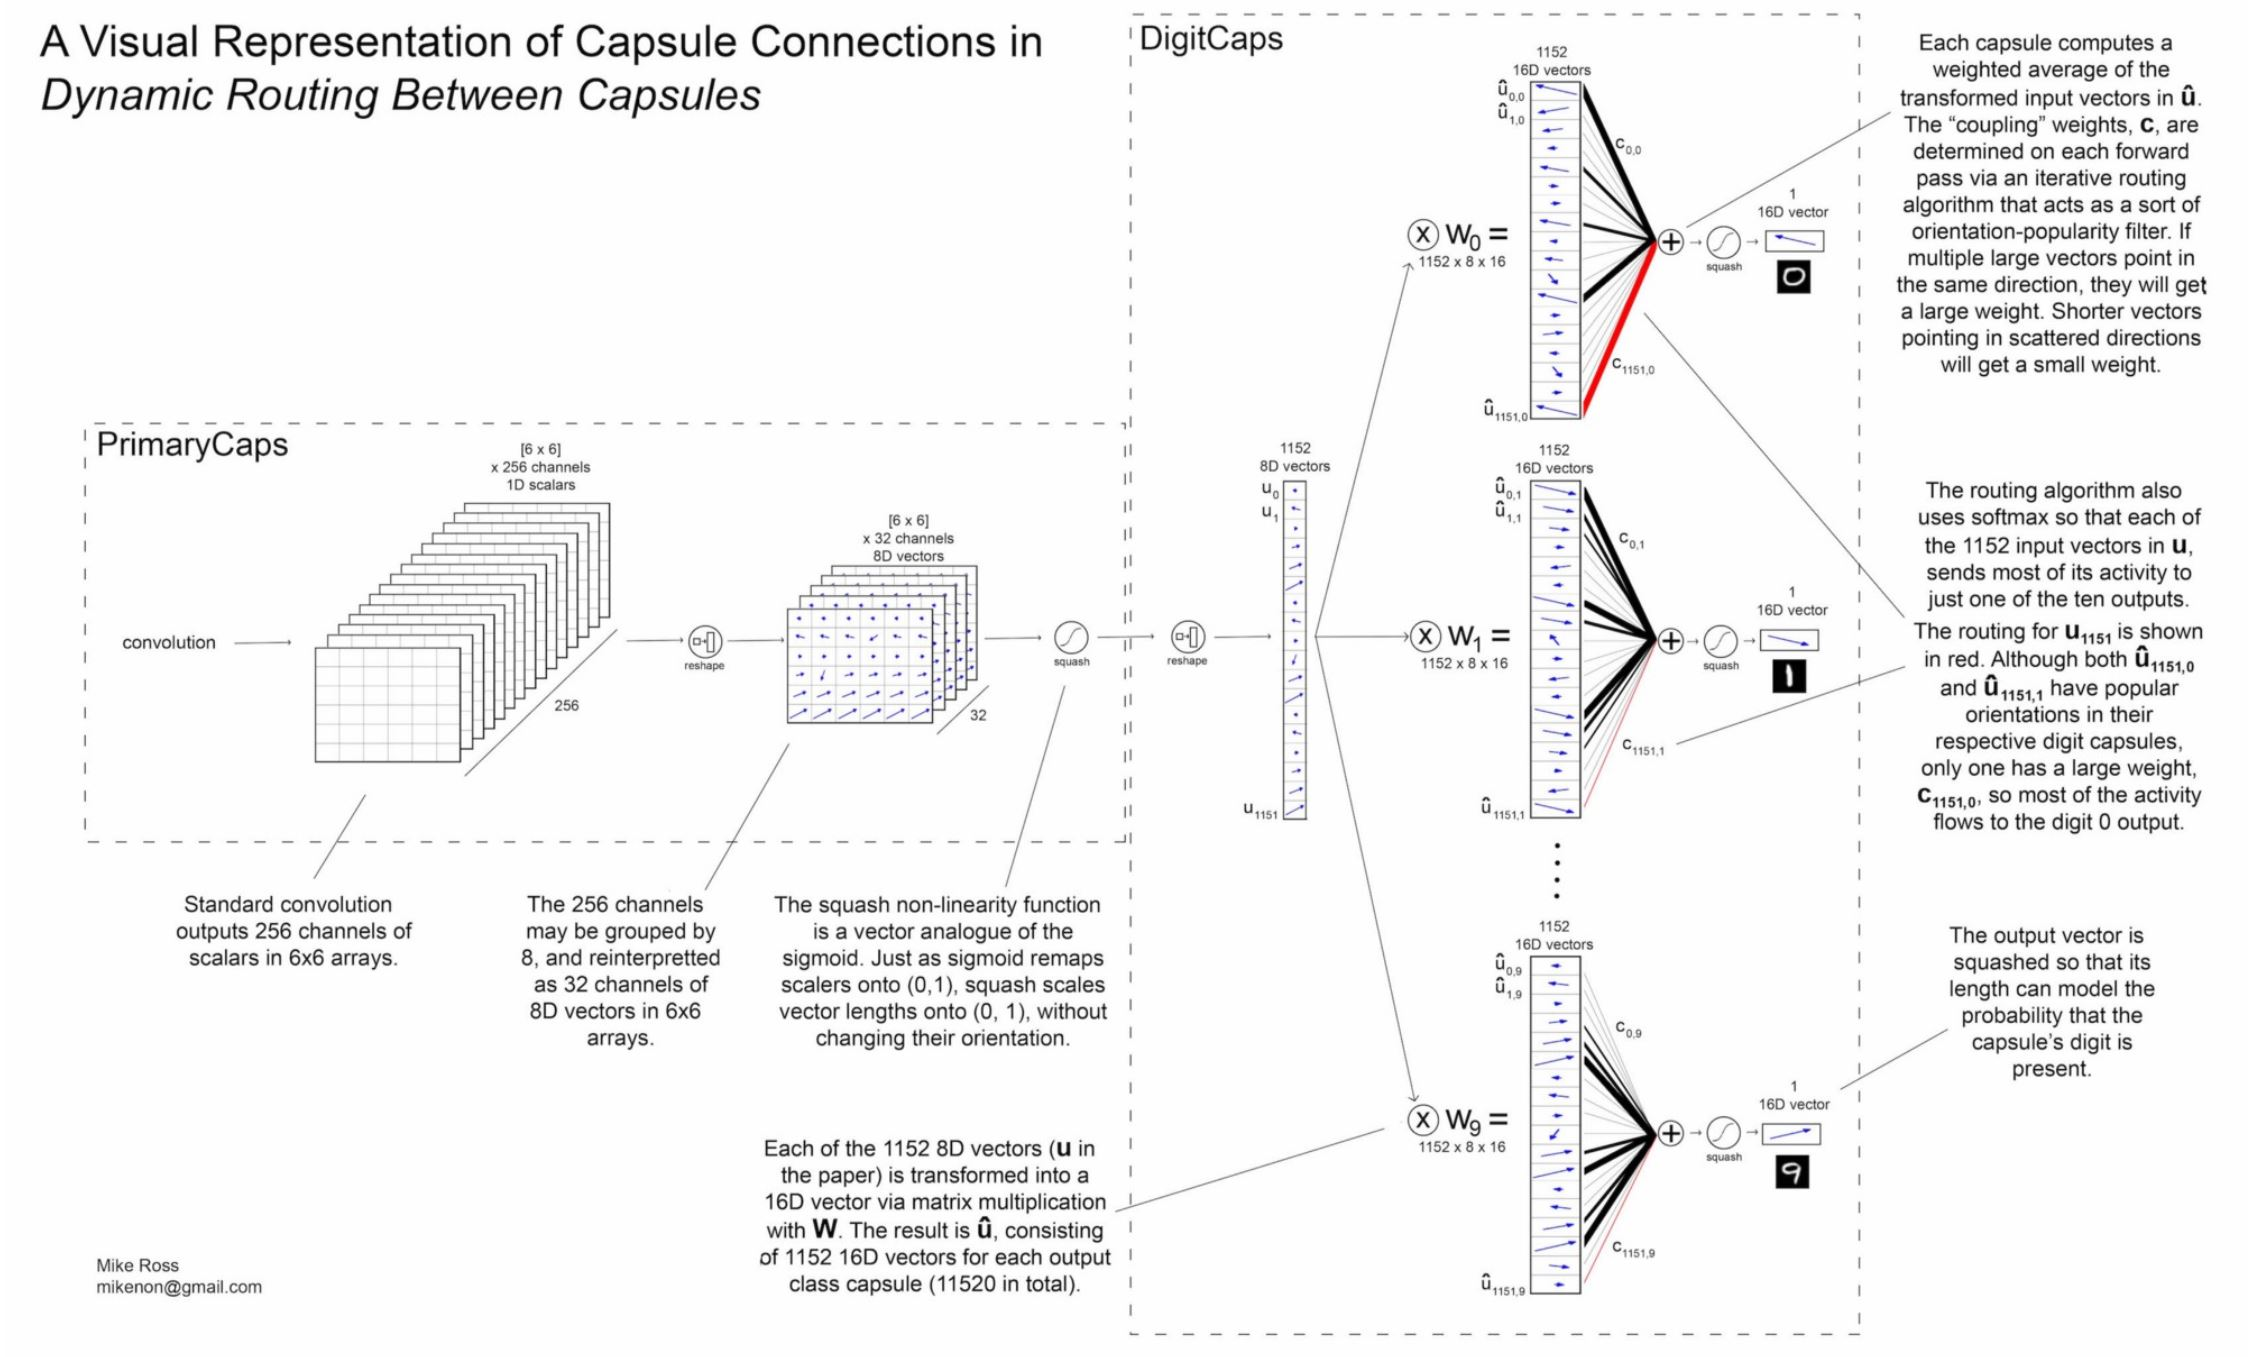
\includegraphics[scale=0.4]{capnet_visual.JPG}
    \end{figure}
\end{frame}

%\subsection{Loss Function for Encoder}
\begin{frame}{Loss Function}
    \begin{figure}
        \centering
        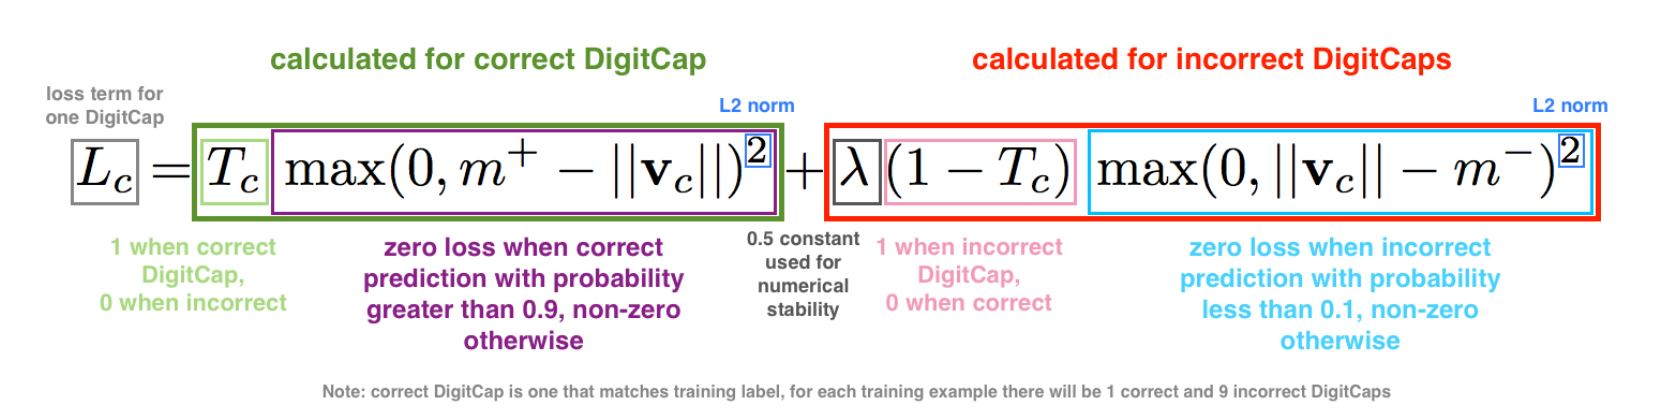
\includegraphics[scale=0.55]{loss.JPG}
    \end{figure}
\end{frame}

\subsection{Capsule Network Decoder Architecture}
\begin{frame}{Capsule Network Decoder Architecture}
    \begin{figure}
        \centering
        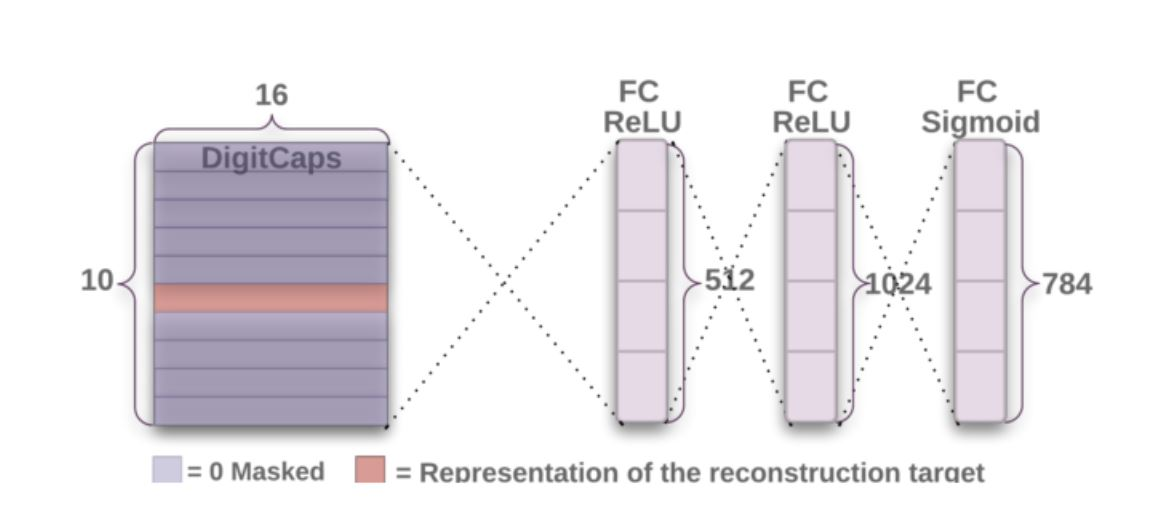
\includegraphics[scale=0.6]{decoder.JPG}
    \end{figure}
    \begin{itemize}
        \item reconstruction loss accounted for by sum of squares between original and predicted intensities
    \end{itemize}
\end{frame}

\section{Experiments and Results}
\subsection{MNIST}
\begin{frame}{Capsules in MNIST and Robustness to Affinity Transformations}
    \begin{itemize}
    \item test errors on 28 x 28 MNIST with 60K and 10K training and testing datasets (with natural variance in skew, rotation, style, etc):
        \begin{figure}
            \centering
            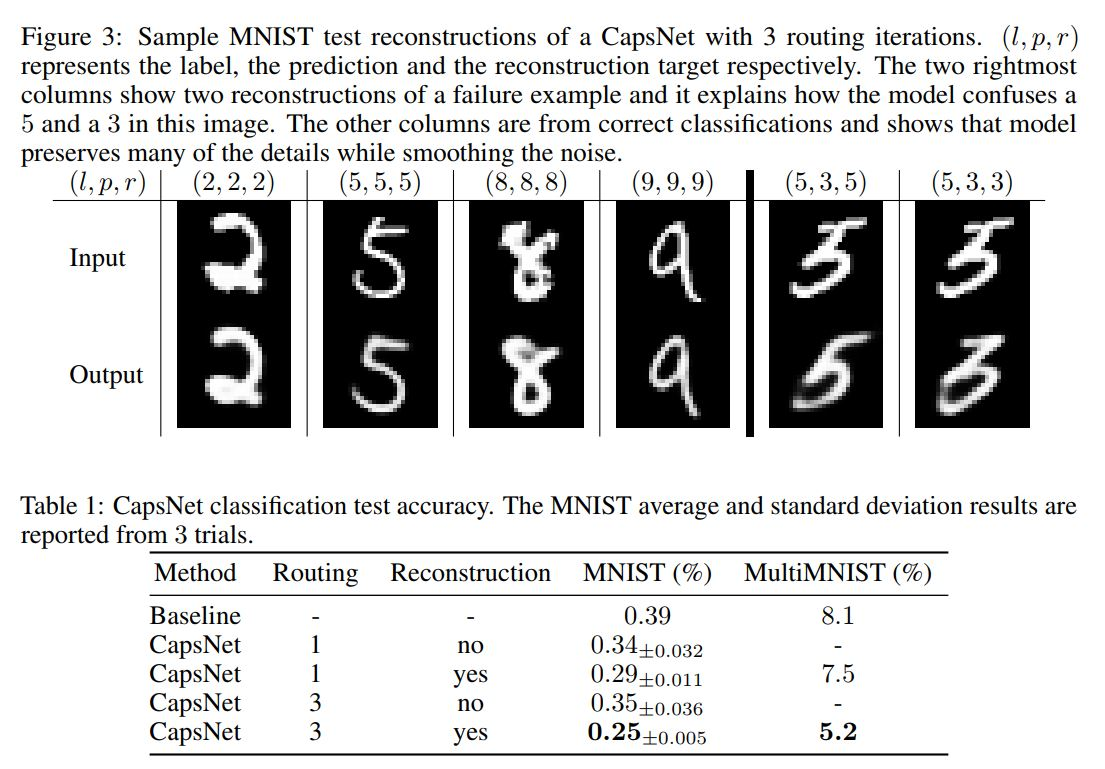
\includegraphics[scale=0.5]{mnist_results.JPG}
        \end{figure}
    
    \end{itemize}
\end{frame}

\begin{frame}{Capsules in MNIST and Robustness to Affinity Transformations}
    \begin{itemize}
        \item tested against traditional CNN with maxpooling and dropout
        \item both trained with MNIST digit placed randomly on a black background of 40 × 40 px
        \item tested on the affNIST
        \item traditional CNN: 99.23\% accuracy on the expanded MNIST test set achieved 79\% accuracy on the affNIST test set
        \item Capsule Network with similar parameters: similar accuracy (99.22\%) on the expanded mnist test set only achieved 66\% on the affNIST test set.
    \end{itemize}
\end{frame}

\subsection{multiMNIST}
\begin{frame}{multiMNIST - Segmenting highly overlapping digits}
\begin{itemize}
    \item Dynamic routing can be viewed as a parallel attention mechanism that allows each capsule at one level to attend to some active capsules at the level below and to ignore others
    \item trained from scratch on the multiMNIST database (Lower L: predicted)
\end{itemize}
\begin{figure}
    \centering
    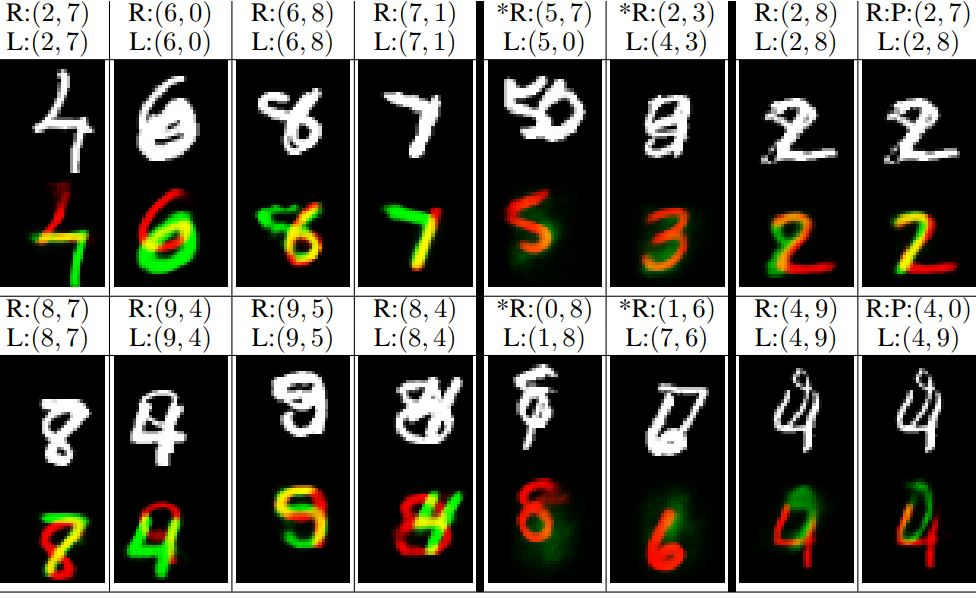
\includegraphics[scale = 0.6]{multiMNIST.JPG}
\end{figure}
\end{frame}

\begin{frame}{multiMNIST - Results}
    \begin{itemize}
        \item Network ability to reconstruct digits regardless of the overlap shows that each digit capsule can pick up the style and position from the votes it is receiving from PrimaryCapsules layer.
    \end{itemize}
    \begin{figure}
        \centering
        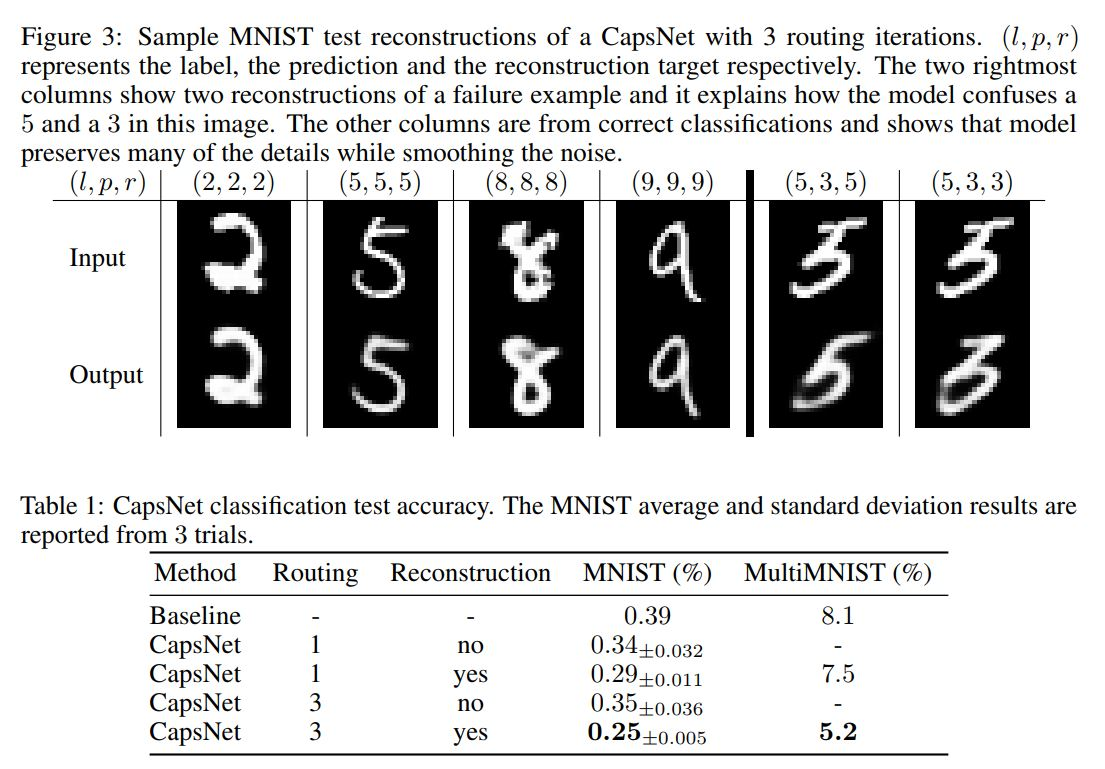
\includegraphics[scale=0.5]{mnist_results.JPG}
    \end{figure}
\end{frame}

\subsection{CIFAR10}
\begin{frame}{CIFAR10}
    \begin{itemize}
        \item CIFAR10 and achieved 10.6\% error with an ensemble of 7 models each of which is trained with 3 routing iterations
        \begin{itemize}
            \item standard CNN achieves 10.6\% error
            \item Each model has the same architecture as the simple model we used for MNIST except that there are three color channels and we used 64 different types of primary capsule
            \item introduced a "none-of-the-above" category for the routing softmaxes, since we do not expect the final layer of ten capsules to explain everything in the image
        \end{itemize}
        \item Drawback: tends to account for everything in the image so it does better when it can model the clutter than when it just uses an additional “orphan” category in the dynamic routing. 
        \begin{itemize}
            \item In CIFAR-10, the backgrounds are much too varied to model in a reasonable sized net which helps to account for the poorer performance.
        \end{itemize}
    \end{itemize}
\end{frame}

\begin{frame}{Thank you for Listening}
    
\end{frame}



% All of the following is optional and typically not needed. 
\appendix
%\section<presentation>*{\appendixname}
\subsection<presentation>*{For Further Reading}

\begin{frame}[allowframebreaks]
  \frametitle<presentation>{For Further Reading}
    
  \begin{thebibliography}{10}
    
  \beamertemplatebookbibitems
  % Start with overview books.

  \bibitem{Author1990}
    Sara Sabour, Nicholas Frosst
Geoffrey E. Hinton.
    \newblock {\em Dynamic Routing Between Capsules}.
    \newblock Google Brain, 2017.
 
    
  \beamertemplatearticlebibitems
  % Followed by interesting articles. Keep the list short. 

  \bibitem{Someone2000}
    S.~Someone.
    \newblock On this and that.
    \newblock {\em Journal of This and That}, 2(1):50--100,
    2000.
  \end{thebibliography}
\end{frame}

\end{document}


